32. \begin{figure}[ht!]
\center{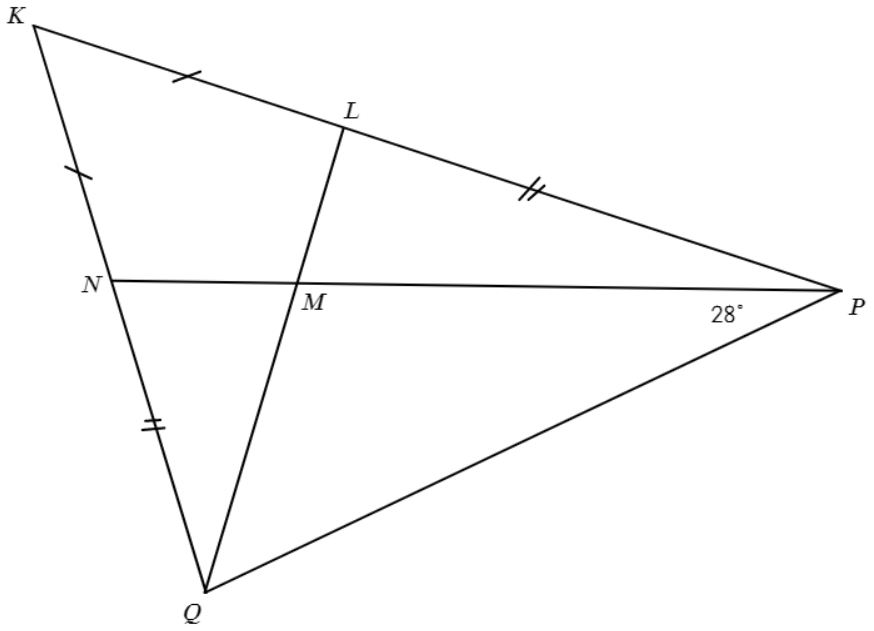
\includegraphics[scale=0.35]{g32.png}}
\end{figure}\\
Заметим, что $NQ=KQ-KN=KP-KL=LP.$ Треугольник $QKP$ является равнобедренным $(KQ=KP),$ значит $\angle KPQ=\angle KQP.$ Тогда
$\left.\begin{array}{l}NQ=LP,\\
\angle NQP=\angle LPQ,\\
QP\text{--- общая.}  \end{array}\right\}\Rightarrow \Delta QNP=\Delta PLQ\text{ по I призн.}$\\$\Rightarrow \angle PQM=\angle PQL=\angle NPQ=\angle MPQ=28^\circ.$\\
